\documentclass{article}

% ------------------------------------ %
%             Document Info            %
% ------------------------------------ %

\usepackage{../../LaTeX-Preamables/Clean}
\newcommand{\documentdate}{Spring 2024}
\newcommand{\documenttype}{Notes}

% ------------------------------------ %
%              Title page              %
% ------------------------------------ %
\begin{document}
\begin{titlepage}
    \null\vfill % Add vertical space to center the title and author

    \centering
    \Huge\textbf{\documentname}

    \vspace{0.1cm}
    \Large\textbf{\documenttype\ $\cdot$ \documentdate}

    \vspace{1cm}
    \normalsize\textbf{Author:} \documentauthor

    \normalsize\textbf{Contact:} \documentauthorcontact

    MORE notes on my \href{https://jaxtam.dev/notes}{website}!
    \vfill % Add vertical space to center the remaining space
    \textcolor{gray}{Made for personal use only. Unmodified re-distribution is allowed. Content for reference only.}
\end{titlepage}

% ------------------------------------ %
%               Document               %
% ------------------------------------ %

\section{Vectors}

\begin{definition}[]{Basics}
  Vector can be represented by $\vec{F}$ or $\boldsymbol{F}$. The magnitude can be represented by $|F|$ or $F$.
\end{definition}

% \begin{definition}[]{Parallelogram law}

%   \begin{tikzpicture}
%     % Define the coordinates
%     \coordinate (O) at (0,0);
%     \coordinate (A) at (2,0);
%     \coordinate (B) at (1,2);
%     \coordinate (C) at ($(A)+(B)$);

%     % Draw the vectors
%     \draw[->] (O) -- (A);
%     \draw[->] (O) -- (B);
%     \draw[->] (O) -- (C);

%     % Draw the parallelogram
%     \draw[dashed] (A) -- (C);
%     \draw[dashed] (B) -- (C);

%     % Label the vectors and points
%     \node[below] at (O) {$O$};
%     \node[below] at (A) {$\mathbf{A}$};
%     \node[left] at (B) {$\mathbf{B}$};
%     \node[above right] at (C) {$\mathbf{A} + \mathbf{B}$};
%   \end{tikzpicture}

%   $\vec{C}=\vec{A}+\vec{B}=\sqrt{A^2+B^2-2AB\cos{\gamma}},\quad\text{where }\gamma=\angle OAC$

% \end{definition}

\begin{knBox}[]{Unit vectors}
  They are vectors with magnitude 1. $\hat{A}=\frac{\vec{A}}{|\vec{A}|}$
\end{knBox}

\subsection{Coplanar vectors}
\begin{definition}
  {Cartesian vector notation}

  In two dimensions, the Cartesian unit vectors $\boldsymbol{i}, \boldsymbol{j}$ are used to designate the directions of the x and y axes respectively.
  \[F=F_x \boldsymbol{i} + F_y \boldsymbol{j}\]
  Where $F_{x/y}$ is the $x/y$ component of $F$. And to find the x/y components we can use trigonometry:
  \[F_x=F\sin{\theta},\quad F_y=F\cos{\theta}\]
\end{definition}

\begin{knBox}
  {Resultant force}
  The resultant force $F_R$ can be found by the sum of the components of $F$:
  \[F_R=\sum F\]
  In Cartesian form, it's the same as adding all the terms together: $F_R=(F_{x1}+F_{x2})\boldsymbol{i}+(F_{y1}+F_{y2})\boldsymbol{j}$
\end{knBox}
\begin{knBox}
  {Orientation of vector}
  We always consider the angle between $F$ \& $F_x$. It can be found by $\theta=\tan^{-1}\frac{F_y}{F_x}$.
\end{knBox}
\begin{knBox}
  {Magnitude of forces}
  The magnitude will simply be the square root of the sum of squared components of the force:
  \[|F|=\sqrt{F_x^2+F_y^2+\dots}\]

\end{knBox}
\subsection{Vectors in 3D}
The concepts above can be extended to 3D simply by adding another variable to the system.
\begin{knBox}
  {Coordinate direction angles in 3D}
  The direction of A is defined by the \emph{coordinate direction angles}: $\alpha, \beta, \gamma$, which are measured between the tail of A and the positive $x, y, z$ axes.
  \[\alpha=\cos^{-1}\frac{A_x}{A},\quad\beta=\cos^{-1}\frac{A_y}{A},\quad\gamma=\cos^{-1}\frac{A_z}{A}\]
  \begin{center}
    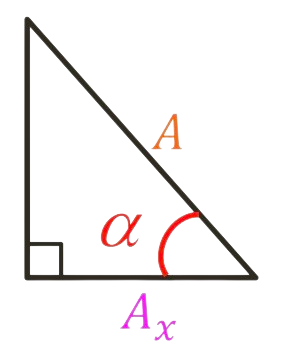
\includegraphics[width=2cm]{img/Ax.png}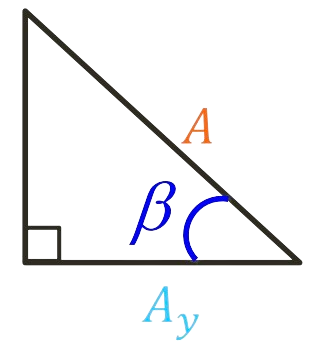
\includegraphics[width=2cm]{img/Ay.png}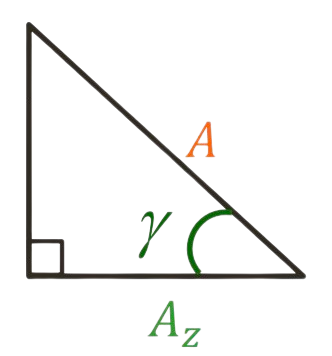
\includegraphics[width=2cm]{img/Az.png}
  \end{center}
\end{knBox}

% TODO: Moving vectors example not right. Also useful for finding resultant vectors, mention this. 
\subsection{Moving vectors}
\begin{definition}
  {Moving vectors by their position vectors}
  We can move a force $F$ to a point using its position vector $r$ (pointing to their tail), using the following definition:
  \[\vec{F}=|F|\times\hat{F}=|F|\times\frac{r}{|r|}\]
  The position vectors are in Cartesian form, so the moved vectors will also be in Cartesian form.
\end{definition}
\subsubsection{Simple example}
\begin{center}
  Consider the following graph:
  \begin{figure}[!ht]
    \centering
    \resizebox{0.15\textwidth}{!}{%
      \begin{circuitikz}
        \tikzstyle{every node}=[font=\normalsize]
        \node [font=\normalsize] at (10.5,10) {F = 100N};
        \draw [->, >=Stealth] (8.25,11) .. controls (9.75,9.75) and (9.75,9.75) .. (11,8.5);
        \draw [dashed] (8.25,11) .. controls (8.25,9.75) and (8.25,9.75) .. (8.25,8.5);
        \draw [dashed] (8.25,8.5) .. controls (9.75,8.5) and (9.75,8.5) .. (11,8.5);
        \node [font=\normalsize] at (7.75,9.5) {4};
        \node [font=\normalsize] at (9.5,8) {4};
        \node [font=\normalsize] at (8.25,11.25) {A};
        \node [font=\normalsize] at (11.25,8.25) {B};
      \end{circuitikz}
    }%
  \end{figure}

  First, we consider $r_{AB}$. From the graph:
  \[\vec{r_{AB}}=4\boldsymbol{i}+4\boldsymbol{j}\]
  Then, we find the magnitude of $r_{AB}$:
  \[|r_{AB}|=\sqrt{4^2+4^2}=5.65\dots\]
  Finally, we apply our formula for $F$:
  \begin{align*}
    \vec{F}=|F|\times\frac{r_{AB}}{|r_{AB}|} & =100\times(\frac{r_x}{5.65}\boldsymbol{i}+\frac{r_y}{5.65}\boldsymbol{j}) \\&=100\times(\frac{4}{5.65}\boldsymbol{i}+\frac{4}{5.65}\boldsymbol{j})\\&=70.7\boldsymbol{i}+70.7\boldsymbol{j}N
  \end{align*}
\end{center}

\section{Moment of forces}
\begin{definition}
  {Definition of moment}
  The moment of a force is a measure of its \emph{tendency} to cause a body to rotate about a specific point.

  The moment about a point $O$, when $F$ is applied a distance $d$ from the point is:
  \[M_O=F\times d\]
  Keep in mind that \emph{positive} moment is \emph{anti-clockwise}.
\end{definition}
\subsection{Coplanar / 2D moment}
\begin{knBox}
  {Resultant moments}
  The resultant moment is the \textbf{sum} of all moments present on the point, given by:
  \[M_R=\sum M_O\]
\end{knBox}
\subsubsection{The moment of a non-linearly attached force}
One simple way is to find the \emph{components} of the force, and sum their individual moments together. The following is a simple example:
\begin{center}
  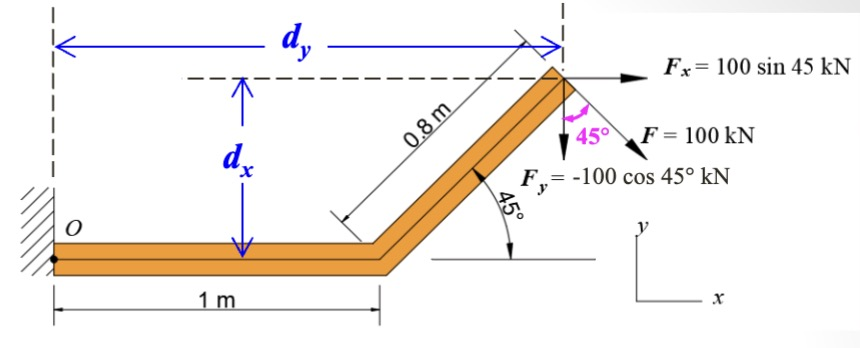
\includegraphics[width=8cm]{img/Moment1.jpg}

  After finding the component forces of $F$, we can deduce the resultant moment to be:
  \begin{align*}
    M_O & =F_x\times 0.8\sin 45\deg+F_y\times(1+0.8\cos 45\deg) \\
        & =-150.7kNm
  \end{align*}
\end{center}

\subsection{Non-coplanar / 3D moment}
\begin{definition}
  {Moments in a 3D system}
  Consider position vector $\vec{r}$ drawn from $O$ to any point on the \emph{line of action} of $F$. The moment can hence be given by:
  \[M_O=r\times F\]
\end{definition}
\begin{definition}
  {Finding the moment via cross products Cartesian vectors}
  The cross product $C$ given by $A$ and $B$ is:
  \[A\times B=\begin{vmatrix}
      i   & j   & k   \\
      A_x & A_y & A_z \\
      B_x & B_y & B_z
    \end{vmatrix}=C\]
  The cross-product for vectors going in the \emph{same direction} is 0. (i.e. $n\boldsymbol{k}\times m\boldsymbol{k}=0$)
\end{definition}
\begin{knBox}
  {Resultant moments}
  The resultant moment is simply the \textbf{sum} of \emph{couple moments} and moments of forces:
  \[(M_R)_O=\sum M_O + \sum M\]
  You can interpret $(M_R)_O$ as the resultant moment about point $O$.
\end{knBox}

\subsection{Couple moments}
Couples are \emph{two parallel forces} that have the same magnitude but have \emph{opposite directions}, separated by a \emph{perpendicular distance} $d$. The magnitude of the moment is given by:
\[M=Fd\]

\begin{minipage}{0.65\textwidth}
  Notice that there's no point mentioned so far. For couple moment, it is \textbf{always the same about any point}. Let's assume for any point $O$ (refer to graph), the moment is:
  \begin{align*}
    M_O & =r_B\times F+r_A\times -F \\&=(r_B-r_A)\times F\\&=r\times F\quad\text{which is independent of }O
  \end{align*}
  Hence, we can say that couple moments are \textbf{free vectors}.
\end{minipage}
\hfill
\begin{minipage}{0.3\textwidth}
  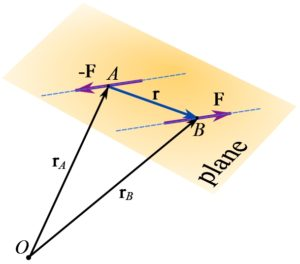
\includegraphics[width=0.95\textwidth]{img/Couple.jpg}
\end{minipage}
% FIXME: This part introduces couples, but what are the actual use cases?

\section{Equilibrium of rigid bodies}

\end{document}